%!tex program = lualatex
\documentclass[answers]{exam}
\usepackage{ctex}
\usepackage{graphicx}
\usepackage[margin=2cm]{geometry}
\usepackage{amsmath, amssymb}
\usepackage{csquotes}
\usepackage{tikz, pgfplots}
\usetikzlibrary{
	angles,
	backgrounds,
	calc,
	decorations.pathmorphing,
	decorations.pathreplacing,
	decorations.text,
	intersections,
	patterns,
	quotes,
	shapes,
	shapes.symbols,
}
\pagestyle{empty}
\newcounter{xcord}
\newcounter{ycord}
\newcounter{total}
\renewcommand{\labelenumi}{\textbf{\ifnum\value{enumi}<10 0\fi\arabic{enumi})}}

\pgfplotsset{compat=1.18}

\CorrectChoiceEmphasis{\color{blue!70!green}\bfseries}
\renewcommand{\solutiontitle}{\textbf{解:}}

\usepackage{array, tabularx}
\newcolumntype{C}{>{\centering\arraybackslash}X}
\newcolumntype{B}{>{\centering\bfseries\arraybackslash}X}
\catcode`\幺=0

\usepackage{tkz-euclide}

\begin{document}
\begin{center}
	\textbf{1997年普通高等学校招生考试(全国卷)}

	\textbf{\Large 理科数学}
\end{center}
\begin{questions}
	\question 设集合$M=\{x|0 \leqslant x < 2\}$,集合$N=\{x|x^2 - 2x - 3 <0\}$,集合$M\cap N=$ \hfill (\hspace{2cm})
	\begin{oneparchoices}
		\choice $\{x|0\leqslant x < 1\}$
		\CorrectChoice $\{x|0\leqslant x < 2\}$
		\choice $\{x|0\leqslant x \leqslant 1\}$
		\choice $\{x|0\leqslant x \leqslant 2\}$
	\end{oneparchoices}

	\begin{solution}
		集合$N=\{x|-1 < x < 3\}$,两个集合的范围如下图所示:

		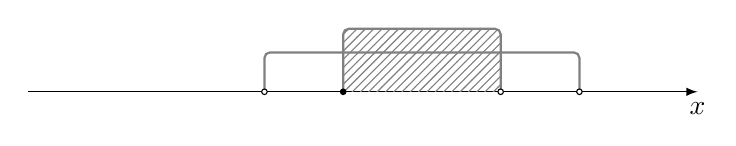
\begin{tikzpicture}
			\tkzInit[xmin=-4, xmax=4]
			\tkzDrawX

			\draw[rounded corners=2pt, thick, black!50] (-1,0) |- (3,.5) -- (3,0);
			\draw[black!50, thick, pattern=north east lines,pattern color=black!50, rounded corners=2pt] (0,0) |- (2,.8) -- (2,0);
			\draw [fill=white](-1,0) circle (1pt);
			\draw [fill=white](3,0) circle (1pt);
			\draw [fill=black](0,0) circle (1pt);
			\draw [fill=white](2,0) circle (1pt);
		\end{tikzpicture}
	\end{solution}

	\question 如果直线$ax+2y+2=0$与直线$3x-y-2=0$平行,那么系数$a=$ \hfs

	\begin{oneparchoices}
		\choice $-3$
		\CorrectChoice $-6$
		\choice $-\dfrac32$
		\choice $\dfrac23$
	\end{oneparchoices}

	\begin{solution}
		两条直线平行则其斜率相等,可得:
		\begin{equation*}
			-\frac{a}{2} = 3
		\end{equation*}
		所以答案为$a=-6$
	\end{solution}

	\question 函数$y=\tan \left( \dfrac12x - \dfrac{\pi}{3} \right)$在一个周期内的图像是 \hfs

	\begin{oneparchoices}
		\pgfplotsset{
			xlabel={$x$},
			ylabel={$y$},
			x label style={at={(current axis.right of origin)}, anchor=north},
			axis lines=center,
			samples=100,
			ticks=none
		}
		\CorrectChoice
		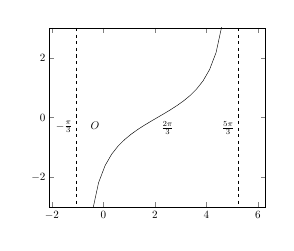
\begin{tikzpicture}[scale=.4]
			\begin{axis}[
					xmin = {-2/3*pi},
					xmax = {2*pi},
					ymin = -3,
					ymax = 3,
				]
				\addplot[domain={-1/3*pi+0.1}:{5/3*pi-0.1}]{tan(deg(1/2*x - pi/3))};
				\draw[dashed] (-pi/3,3) -- (-pi/3, -3);
				\draw[dashed] (pi*5/3,3) -- (pi*5/3, -3);
				\node[below left] at (-pi/3, 0) {$-\frac{\pi}{3}$};
				\node[below right] at (2*pi/3, 0) {$\frac{2\pi}{3}$};
				\node[below left] at (5*pi/3, 0) {$\frac{5\pi}{3}$};
				\node[below left] at (0,0) {$O$};
			\end{axis}
		\end{tikzpicture}
		\choice
		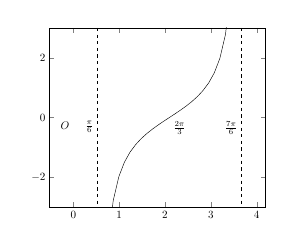
\begin{tikzpicture}[scale=.4]
			\begin{axis}[
					xmin = {-1/6*pi},
					xmax = {8/6*pi},
					ymin = -3,
					ymax = 3,
				]
				\addplot[domain={1/6*pi+0.1}:{7/6*pi-0.1}]{tan(deg(x - 2/3*pi))};
				\draw[dashed] (pi/6,3) -- (pi/6, -3);
				\draw[dashed] (pi*7/6,3) -- (pi*7/6, -3);
				\node[below left] at (pi/6, 0) {$\frac{\pi}{6}$};
				\node[below right] at (2*pi/3, 0) {$\frac{2\pi}{3}$};
				\node[below left] at (7*pi/6, 0) {$\frac{7\pi}{6}$};
				\node[below left] at (0,0) {$O$};
			\end{axis}
		\end{tikzpicture}
		\choice
		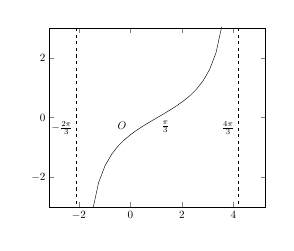
\begin{tikzpicture}[scale=.4]
			\begin{axis}[
					xmin = {-pi},
					xmax = {5/3*pi},
					ymin = -3,
					ymax = 3,
				]
				\addplot[domain={-2/3*pi+0.1}:{4/3*pi-0.1}]{tan(deg(1/2*x - pi/6))};
				\draw[dashed] (-pi*2/3,3) -- (-pi*2/3, -3);
				\draw[dashed] (pi*4/3,3) -- (pi*4/3, -3);
				\node[below left] at (-pi*2/3, 0) {$-\frac{2\pi}{3}$};
				\node[below right] at (pi/3, 0) {$\frac{\pi}{3}$};
				\node[below left] at (4*pi/3, 0) {$\frac{4\pi}{3}$};
				\node[below left] at (0,0) {$O$};
			\end{axis}
		\end{tikzpicture}
		\choice
		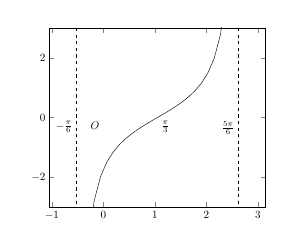
\begin{tikzpicture}[scale=.4]
			\begin{axis}[
					xmin = {-1/3*pi},
					xmax = {pi},
					ymin = -3,
					ymax = 3,
				]
				\addplot[domain={-1/6*pi+0.1}:{5/6*pi-0.1}]{tan(deg(x - 1/3*pi))};
				\draw[dashed] (-pi/6,3) -- (-pi/6, -3);
				\draw[dashed] (pi*5/6,3) -- (pi*5/6, -3);
				\node[below left] at (-pi/6, 0) {$-\frac{\pi}{6}$};
				\node[below right] at (pi/3, 0) {$\frac{\pi}{3}$};
				\node[below left] at (5*pi/6, 0) {$\frac{5\pi}{6}$};
				\node[below left] at (0,0) {$O$};
			\end{axis}
		\end{tikzpicture}
	\end{oneparchoices}
	\begin{solution}
		$\tan{x}$的周期是$\pi$,所以$\tan{\frac12{x}}$的周期应该为$2\pi$.因此排除B和D.
		$\tan(\frac12\cdot\frac{\pi}{3}-\frac{\pi}{3}) \neq 0$,因此选A.
	\end{solution}
	\question
	已知三棱锥$D-ABC$的三个侧面与底面全等,且$AB=AC=\sqrt{3}$,$BC=2$,则以$BC$为棱,以面$BCD$与面$BCA$为面的二面角的大小是
	\hfs

	\begin{oneparchoices}
		\choice $\arccos\dfrac{\sqrt{3}}{3}$
		\choice $\arccos\dfrac{1}{3}$
		\CorrectChoice $\dfrac{\pi}{2}$
		\choice $\dfrac{2\pi}{3}$
	\end{oneparchoices}

	\begin{solution}

		\tdplotsetmaincoords{20}{120}
		\begin{center}
			\begin{tikzpicture}[tdplot_main_coords, baseline=(current bounding box.north)]
				\coordinate(A) at ({sqrt(2)}, 0);
				\coordinate(B) at (0,1);
				\coordinate(C) at (0,-1);
				\coordinate(D) at (0,0,{sqrt(2)});

				\draw(A)node[below]{$A$} -- (B)node[below]{$B$};
				\draw[dashed](B)-- (C)node[above]{$C$};
				\draw(C)-- (A);
				\draw(D)node[above]{$D$} -- (A);
				\draw(D) -- (B);
				\draw(D) -- (C);

				\draw[blue, dashed](A) -- (0,0)node[below right]{$O$} -- (D);
			\end{tikzpicture}
		\end{center}

		取$BC$的中点为$O$,连接$AO$和$DO$.
		因为$AC=AB$,所以有$AO\perp BC$.因为$\triangle{BCD}\cong\triangle{BCA}$,所以也有$DO\perp
			BC$.计算可得$AO=DO=\sqrt{2}$.另外有$AD=2$.可以看出有$AO^2 + DO^2 =
			AD^2$,所以$\triangle{AOD}$是直角三角形,即二面角为$\ang{90}$.
	\end{solution}

	\question 函数$y=\sin \left( \dfrac{\pi}{3} - 2x \right) + \cos2x$的最小正周期是 \hfs

	\begin{oneparchoices}
		\choice $\dfrac{\pi}{2}$
		\CorrectChoice $\pi$
		\choice $2\pi$
		\choice $\dfrac{2\pi}{3}$
	\end{oneparchoices}

	\begin{solution}
		因为$\sin \left( \dfrac{\pi}{3} -2x \right)$与$\cos2x$的周期均为$\pi$,所以函数的最小正周期也为$\pi$.
	\end{solution}

	\question 满足$\arccos(1-x) \geqslant \arccos{x}$的取值范围是 \hfs

	\begin{oneparchoices}
		\choice $\left[-1, -\dfrac12\right]$
		\choice $\left[-\dfrac12, 0\right]$
		\choice $\left[0, \dfrac12\right]$
		\CorrectChoice $\left[\dfrac12, 1\right]$
	\end{oneparchoices}

	\begin{solution}
		因为$\arccos$的定义域是$[-1,1]$,所以排队选项A和B.

		$\arccos(0) = \frac{\pi}{2}, \arccos(1-0)=0$,所以C也可以排除.答案为D.
	\end{solution}

	\question 将$y=2^x$的图像\underline{\hspace{.5cm}},再作关于直线$y=x$对称的图像,可得到函数$y=\log_2(x+1)$的图像. \hfs

	\begin{oneparchoices}
		\choice 先向左平移$1$个单位
		\choice 先向右平移$1$个单位
		\choice 先向上平移$1$个单位
		\CorrectChoice 先向下平移$1$个单位
	\end{oneparchoices}

	\begin{solution}
		点$(0,0)$在直线$y=x$上,并且也在函数$y=\log_2(x+1)$上,所以应该也在$y=2^x$平移后的图像上,可以得到平移后的图像为$y=2^x
			- 1$才能满足点$(0,0)$在图像上.
	\end{solution}

	\question 长方体一个顶点上三条棱的长分别是$3,4,5$,且它的八个顶点都在同一个球面上,这个球的表面积是

	\hfs

	\begin{oneparchoices}
		\choice $20\sqrt{2}\pi$
		\choice $25\sqrt{2}\pi$
		\choice $50\pi$
		\choice $200\pi$
	\end{oneparchoices}

	\begin{solution}

		\tdplotsetmaincoords{60}{120}
		\begin{center}
			\begin{tikzpicture}[tdplot_main_coords]
				\coordinate (A) at (0,0);
				\coordinate (B) at (3,0);
				\coordinate (C) at (3,4);
				\coordinate (D) at (0,4);
				\coordinate (A') at (0,0,5);
				\coordinate (B') at (3,0,5);
				\coordinate (C') at (3,4,5);
				\coordinate (D') at (0,4,5);

				\draw (B) -- (C) -- (D);
				\draw[dashed] (A) -- (B) (D) -- (A);
				\draw (A') -- (B') -- (C') -- (D') -- cycle;
				\draw[dashed] (A) -- (A');
				\draw (B) -- (B');
				\draw (C) -- (C');
				\draw (D) -- (D');
				\draw[dashed] (A) -- (C');
				\draw[dashed] (A) -- (C);

				\tkzLabelPoint[left](A){$A$}
				\tkzLabelPoint[left](B){$B$}
				\tkzLabelPoint[below](C){$C$}
				\tkzLabelPoint[above](C'){$C'$}
			\end{tikzpicture}
		\end{center}

		\begin{align*}
			AB = 3, BC = 4, CC'= 5             \\
			AC = \sqrt{3^2 + 4^2} = 5          \\
			AC' = \sqrt{5^2 + 5^2} = 5\sqrt{2} \\
		\end{align*}
		则球体的半径为$\frac12AC'=\frac{5\sqrt{2}}{2}$, 球体的表面积为$4\pi \left( \frac{5\sqrt{2}}{2} \right)^2=50\pi$.
	\end{solution}

	\question 曲线的参数方程是\begin{math}
		\begin{cases}
			x = 1 - \dfrac1t \\
			y = 1 - t^2
		\end{cases}(t是参数,t\neq0),它的普通方程是 \hfs
	\end{math}

	\begin{oneparchoices}
		\choice $(x-1)^2(y-1)=1$
		\CorrectChoice $y=\dfrac{x(x-2)}{(1-x)^2}$
		\choice $y=\dfrac{1}{(1-x)^2} -1$
		\choice $y=\dfrac{x}{1-x^2} + 1$
	\end{oneparchoices}

	\begin{solution}
		由$x = 1 - \dfrac1t$得$t=\dfrac{1}{1-x}$,代入$y=1-t^2$得
		\begin{align*}
			y & = 1- \frac{1}{(1-x)^2}           \\
			  & = \frac{1-2x + x^2 - 1}{(1-x)^2} \\
			  & = \frac{x(x-2)}{(1-x)^2}
		\end{align*}
	\end{solution}

	\question 函数$y=\cos^2x-3\cos{x} + 2$的最小值为 \hfs

	\begin{oneparchoices}
		\choice $2$
		\CorrectChoice $0$
		\choice $-\dfrac14$
		\choice $6$
	\end{oneparchoices}

	\begin{solution}
		\begin{align*}
			y & = \cos^2x - 3x + \frac94 - \frac14 \\
			  & = (\cos{x} - \frac32)^2 - \frac14  \\
		\end{align*}
		$(\cos{x}-\dfrac32)^2$最小值为$\dfrac14$,则函数的最小值为$0$.
	\end{solution}

	\question 椭圆$C$与椭圆$\dfrac{(x-3)^2}{9} + \dfrac{(y-2)^2}{4}=1$关于直线$x+y=0$对称,椭圆$C$的方程是 \hfs

	\begin{choices}
		\CorrectChoice $\dfrac{(x+2)^2}{4} + \dfrac{(y+3)^2}{9} = 1$
		\choice $\dfrac{(x-2)^2}{9} + \dfrac{(y-3)^2}{4} = 1$
		\choice $\dfrac{(x+2)^2}{9} + \dfrac{(y+3)^2}{4} = 1$
		\choice $\dfrac{(x-2)^2}{4} + \dfrac{(y-3)^2}{9} = 1$
	\end{choices}

	\begin{solution}
		对于椭圆$C$上的任一点$(x,y)$,其关于直线$x+y=0$对称的点为$(-y, -x)$,代入椭圆方程得:
		\begin{align*}
			\frac{(-y-3)^2}{9} + \frac{(-x-2)^2}{4} & = 1 \\
			\frac{(y+3)^2}{9} + \frac{(x+2)^2}{4}   & = 1
		\end{align*}
	\end{solution}

	\question 圆台上、下底面积分别为$\pi$、$4\pi$,侧面积为$6\pi$,这个圆台的体积是\hfs

	\begin{oneparchoices}
		\choice $\dfrac{2\sqrt{3}\pi}{3}$
		\choice $2\sqrt{3}\pi$
		\choice $\dfrac{7\sqrt{3}\pi}{6}$
		\CorrectChoice $\dfrac{7\sqrt{3}\pi}{3}$
	\end{oneparchoices}

	\begin{solution}
		\tdplotsetmaincoords{80}{0}
		\begin{center}
			\begin{tikzpicture}[tdplot_main_coords]
				\draw[dashed] (2,0) arc (0:180:2);
				\draw (2,0) arc (0:-180:2);
				\draw (0,0,1) circle(1);

				\draw[thin] (2,0,0) -- node[above, sloped]{$l$}(1,0,1);
				\draw[thin] (-2,0,0) -- (-1,0,1);

				\draw (0,0,1)node[left]{$r_2$} -- (1,0,1);
				\draw[dashed] (0,0)node[left]{$r_1$} -- (2,0);
				\draw[dashed] (0,0) -- (0,0,2);
				\draw[dashed] (0,0,2) --node[above, sloped]{$l'$} (1,0,1);
			\end{tikzpicture}
		\end{center}

		圆台的侧面积$=\pi(l+l')r_1 - \pi l'r_2$,而$\frac{l'}{l'+l}=\frac{r_2}{r_1}=\frac12$,即$l'=l$,代入面积公式中得:
		$3\pi l = 6\pi$,得到$l=2$.圆台的高$h=\sqrt{l^2-(r_1-r_2)^2}=\sqrt{3}$.
		\begin{align*}
			V & = \frac13h{(S_上 + S_下 + \sqrt{S_上S_下})} \\
			  & = \frac{7\sqrt{3}\pi}{3}
		\end{align*}
	\end{solution}

	\question
	定义在区间$(-\infty,+\infty)$的奇函数$f(x)$为增函数,偶函数$g(x)$在区间$[0,+\infty)$的图像与$f(x)$的图像重合,设$a>b>0$,给出下列不等式:

	\circled{1}$f(b)-f(-a)>g(a)-g(-b)$; \circled{2}$f(b)-f(-a) < g(a) - g(-b)$;
	\circled{3}$f(a)-f(-b) > g(b) - g(-a)$; \circled{4}$f(a)-f(-b) < g(b) - g(-a)$.
	其中成立的是 \hfs

	\begin{oneparchoices}
		\choice \circled{1}与\circled{4}
		\choice \circled{2}与\circled{3}
		\CorrectChoice \circled{1}与\circled{3}
		\choice \circled{2}与\circled{4}
	\end{oneparchoices}

	\begin{solution}
		\begin{enumerate}[label=\protect\circled{\arabic*}]
			\item $f(b) - f(-a) = f(b)+f(a)$, $g(a) - g(-b) = g(a) - g(b)$,所以有$f(b)-f(-a) > g(a) - g(-b)$;
			\item 不成立;
			\item $f(a) - f(-b) = f(a) + f(b)$, $g(b) - g(-a)= g(b) - g(a)$,所以有$f(a) - f(-b) > g(b) - g(-a)$
			\item 不成立
		\end{enumerate}
	\end{solution}

	\question 不等式组 \begin{math}
		\begin{cases}
			x> 0 \\
			\dfrac{3-x}{3+x} > \left|\dfrac{2-x}{2+x}\right|
		\end{cases}
	\end{math}的解集是 \hfs

	\begin{oneparchoices}
		\choice $\{x|0< x < 2\}$
		\choice $\{x|0< x < 2.5\}$
		\CorrectChoice $\{x|0< x < \sqrt{6}\}$
		\choice $\{x|0< x < 3\}$
	\end{oneparchoices}

	\begin{solution}
		从\begin{math}
			\begin{cases}
				x> 0 \\
				\dfrac{3-x}{3+x} > \left|\dfrac{2-x}{2+x}\right|
			\end{cases}
		\end{math}可得
		\begin{align*}
			\frac{3-x}{3+x} & > \frac{2-x}{2+x} \qquad (-2 < x \leqslant 2) \tag{1}          \\
			\frac{3-x}{3+x} & > \frac{x-2}{2+x}  \qquad (-2 > x(x\neq-3) \cup x > 2) \tag{2}
		\end{align*}
		由式$(1)$得
		\begin{align*}
			6+x-x^2> 6-x -x^2 \qquad (-2 \leqslant x \leqslant 2) \\
			0 < x \leqslant 2 \tag{a}
		\end{align*}
		由式$(2)$得
		\begin{align*}
			6 +x - x^2 > -6 +x + x^2 \qquad (-2 > x(x\neq-3) \cup x > 2) \\
			6 > x^2 \qquad (-2 > x (x\neq-3) \cup x > 2)                 \\
			-\sqrt{6} < x < -2, 2 < x < \sqrt{6} \tag{b}
		\end{align*}
		综合$(a)$和$(b)$可得 $-\sqrt{6}<x < -2, 0< x <
			\sqrt{6}$,再结合题目中$x>0$的条件,所以最后的解集是$\{x|0<x<\sqrt{6}\}$
	\end{solution}

	\question 四面体的顶点和各棱中点共$10$个点,在其中取$4$个不共面的点,不同的取法共有 \hfs

	\begin{oneparchoices}
		\CorrectChoice $150$种
		\choice $147$种
		\choice $144$种
		\choice $141$种
	\end{oneparchoices}

	\begin{solution}
		从$10$个点中取$4$个点一共有$\binom{10}{4}=\frac{10\times9\times8\times7}{4\times3\times2\times1}=210$种.四面体上一个面上有规定的$6$个点,从这$6$个点中取$4$个点的取法有$\binom{6}{4}=15$种,一共有$4$个面,所以取得在同一个面上的$4$个点的取法有$60$种.则取$4$个不共面的点的取法共有$150$种.
	\end{solution}

	\question 已经$\left( \dfrac{a}{x} -\sqrt{\dfrac{x}{2}}
		\right)^9$的展开式中$x^3$的系数为$\frac94$,常数$a$的值为\fillin[36][2cm].

	\begin{solution}
		\begin{align*}
			\left( \frac{a}{x} - \sqrt{\frac{x}{2}} \right)^9
			 & = \sum_{r=0}^9\binom{9}{r} \left( \frac{a}{x} \right)^{9-r} \left( -\sqrt{\frac{x}{2}} \right)^r \\
			 & = \sum_{r=0}^{9}\binom{9}{r} a^{9-r}(-1)^r2^{-\frac{r}{2}}x^{r-9 + \frac{r}{2}}
		\end{align*}
		$x$的指数为$3$时有$r-9+\frac{r}{2} = 3$,计算得$r=8$.此时系数为$a^{9-8}(-1)^82^{-\frac{8}{2}} = \frac94$.

		$a=36$.
	\end{solution}
	\question 已知直线的极坐标方程为$\rho\sin \left( \theta + \dfrac{\pi}{4} \right) =
		\dfrac{\sqrt{2}}{2}$,则极点到该直线的距离是 \fillin[$\dfrac{\sqrt{2}}{2}$][2cm].

	\begin{solution}
		\begin{align*}
			\rho\sin \left( \theta + \frac{\pi}{4} \right)
			 & = \rho( \sin\theta\cos\frac{\pi}{4} + \cos\theta\sin\frac{\pi}{4}) \\
			 & =  \frac{\sqrt{2}}{2}\rho(\sin\theta + \cos\theta)                 \\
			 & = \frac{\sqrt{2}}{2}
		\end{align*}
		所以极坐标方程可以化简为:
		\begin{equation*}
			\rho\sin\theta + \rho\cos\theta = 1
		\end{equation*}
		将$x=\cos\theta, y=\sin\theta$代入极坐标方程可得直线的直角坐标方程为
		\begin{equation*}
			x + y - 1 = 0
		\end{equation*}
		任意一点$(x_1, y_1)$到直线$Ax+By+C=0$的距离为:
		\begin{align*}
			d = \frac{|Ax_1+By_1+C|}{\sqrt{A^2+B^2}}
		\end{align*}
		将$A=1,B=1,C=-1,x_1=0, y_1=0$代入得
		\begin{align*}
			d = \frac{1}{\sqrt{2}} = \frac{\sqrt{2}}{2}
		\end{align*}
	\end{solution}

	\question
	$\dfrac{\sin{\ang{7}}+\cos{\ang{15}}\sin{\ang{8}}}{\cos{\ang{7}}-\sin{\ang{15}}\sin{\ang{8}}}$的值为\fillin[$2-\sqrt{3}$][2cm].

	\begin{solution}
		\begin{align*}
			\frac{\sin{\ang{7}}+\cos{\ang{15}}\sin{\ang{8}}}{\cos{\ang{7}}-\sin{\ang{15}}\sin{\ang{8}}}
			 & = \frac{\sin(\ang{15}-\ang{8}) + \cos\ang{15}\sin\ang8}{\cos(\ang{15}-\ang8) -\sin\ang{15}\sin\ang8} \\
			 & = \frac{\sin\ang{15}\cos8 - \cos\ang{15}\sin\ang8 + \cos\ang{15}\sin\ang8}
			{\cos\ang{15}\cos8 + \sin\ang{15}\sin\ang8 - \sin\ang{15}\sin\ang8}                                     \\
			 & = \frac{\sin\ang{15}}{\cos\ang{15}}                                                                  \\
			 & = \tan\ang{15}                                                                                       \\
			 & = \frac{\sin\ang{30}}{1+\cos\ang{30}}                                                                \\
			 & = \frac{\frac12}{1+\frac{\sqrt{3}}{2}}                                                               \\
			 & = 2 - \sqrt{3}
		\end{align*}
	\end{solution}
\end{questions}
\end{document}
